\section{Systemarchitektur}

\subsection{Grobentwurf}

\begin{figure} 
  \centering
     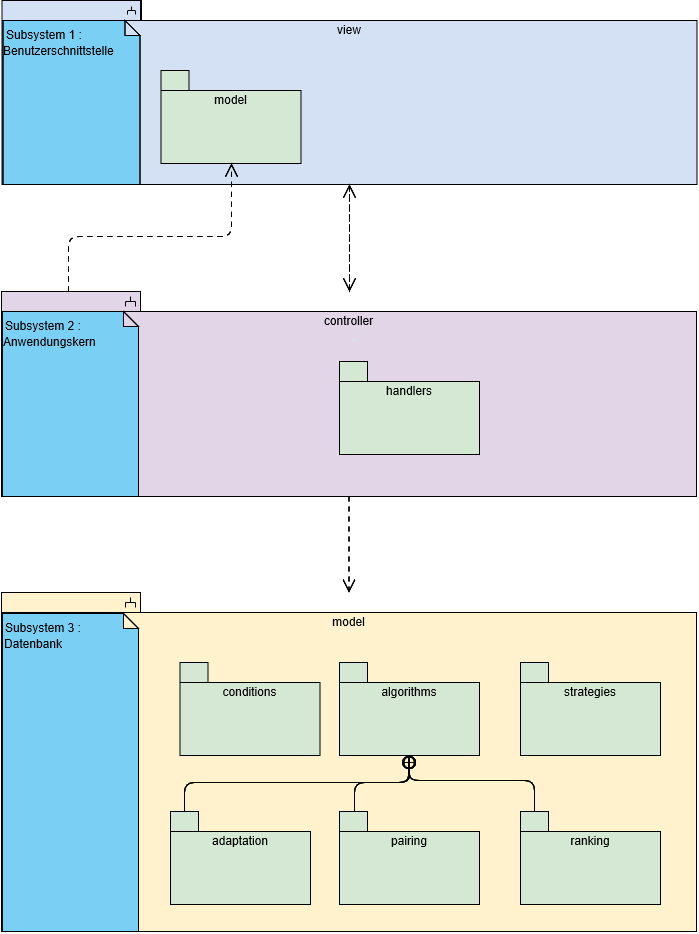
\includegraphics[width=1.1\textwidth]{UMLzuGrobentwurf}
\end{figure}

Sswis baut auf einem MVC-Model auf, welches um ein ViewModel erweitert wurde, was ein vollständiges Abkoppeln von Model und View ermöglicht.
Die Benutzerinteraktion erfolgt über die View. Im ViewModel werden die Benutzereingaben zwischengespeichert und auf Korrektheit überprüft. Des Weiteren schreibt der Controller diejenigen Informationen in das ViewModel, die auf der Benutzeroberfläche angezeigt werden sollen.\\
Der Controller ist für die Programmflusssteuerung zuständig. Die ActionListener der Benutzeroberfläche sind im Controller implementiert. Hierdurch können etwa neue Benutzeroberflächen unter Wiederverwendung der ActionListener erstellt werden.
Außerdem dient der Controller zur Kommunikation zwischen View und Model.\\
Im Model sind die Objekte der Simulation abgebildet. Auch ist hier die gesamte Business Logic implementiert.

\subsection{Controller}

\noindent
\makebox[\textwidth]{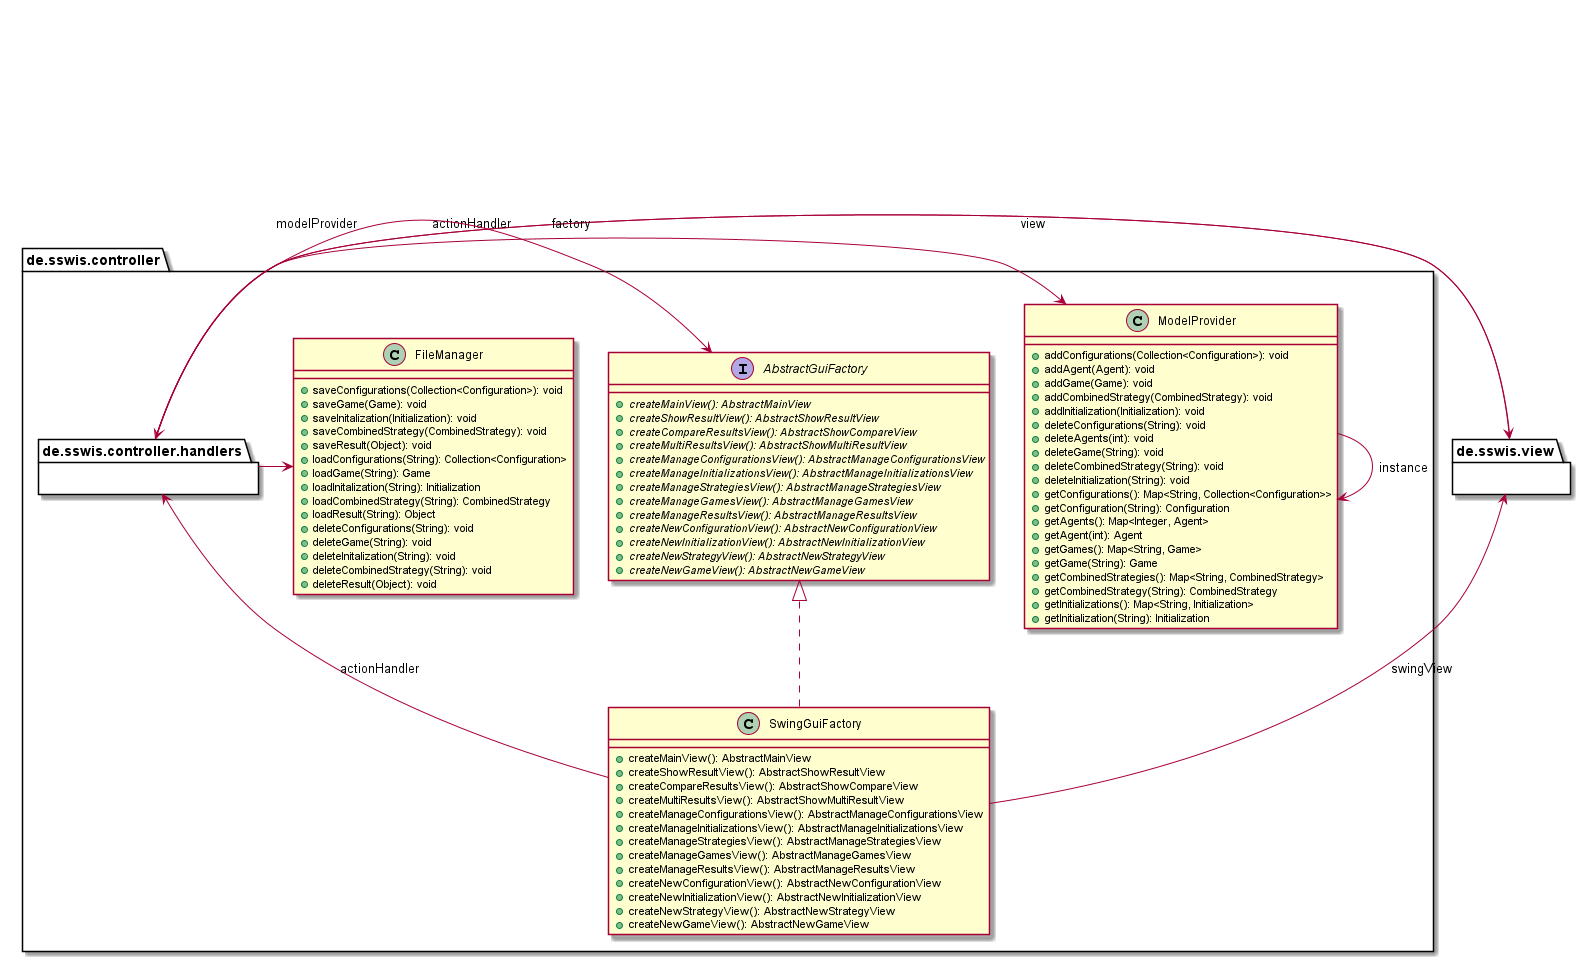
\includegraphics[scale=0.36]{Controller_package}}

Zur Erfüllung der oben angedeuteten Aufgaben steht dem Controller eine Reihe an weiteren Klassen neben den ActionListener-Klassen, die sich im Paket Handlers befinden, zur Verfügung.\\
Zum einen müssen die GUI-Objekte, d.h. alle Fenster mit denen der Benutzer interagiert, erstellt werden. Dies wird durch das Fabrik-Entwurfsmuster realisiert. Das AbstractGuiFactory-Interface gibt alle nötigen Ansichten vor und bietet weiterhin die oben beschriebene Möglichkeit, das Programm zu einem späteren Zeitpunkt komfortabel um neue Benutzeroberflächen zu erweitern.\\
Die SwingGuiFactory-Klasse erstellt die Objekte der von diesem Entwicklerteam angebotenen, Swing-basierten Benutzeroberfläche.

Bei dem ModelProvider handelt es sich um ein Einzelstück, das als zentrale Anlaufstelle für alle Model-Objekte dient. Das Einzelstück-Entwurfsmuster wurde verwendet, um Inkonsistenzen vorzubeugen.

Im FileManager werden Methoden zum Speichern, Laden und Löschen von Objekten bereitgestellt, die gesicherte Benutzereingaben und Ergebnisse darstellen. Das Bearbeiten dieser Objekte geschieht durch ein Laden und anschließendes Speichern des gegebenen Objekts.\\
Die Objekte werden in einem programminternen Verzeichnis gespeichert.

Die vom Programm angebotenen "Dienstleistungen", darunter fallen die diversen Algorithmentypen\footnote{Adaptionsalgorithmen, Paarungsalgorithmen und Bewertungsalgorithmen} sowie die verfügbaren Bedingungen und Basis-Strategien, können durch den ModelServiceLoader zur Verfügung gestellt werden.\\
Dies ist nötig, da sie auf Entwicklerebene um weitere Ausprägungen ergänzt werden können und diese ebenfalls an allen relevanten Stellen, z.B. im Auswahlfenster für den Benutzer, sichtbar sein sollen.

Der ModelParser überträgt das ViewModel in das Model. Konkret werden die im ViewModel auf Korrektheit überprüften Benutzereingaben in Objekte umgewandelt, mit denen eine Simulation durchgeführt werden kann. Andersherum werden die Daten abgelaufener Simulationen in ein Format konvertiert, das die View darstellen kann.

Schließlich können durch das Interface Simulationen überwacht werden, wobei der ViewNotifier die Benutzeroberfläche benachrichtigt, sobald eine Simulation abgeschlossen ist. Es findet eine Parallelisierung statt, wodurch die Benutzeroberfläche auch während einer Simulation aktiv bleibt.

\subsection{Model}

\noindent
\makebox[\textwidth]{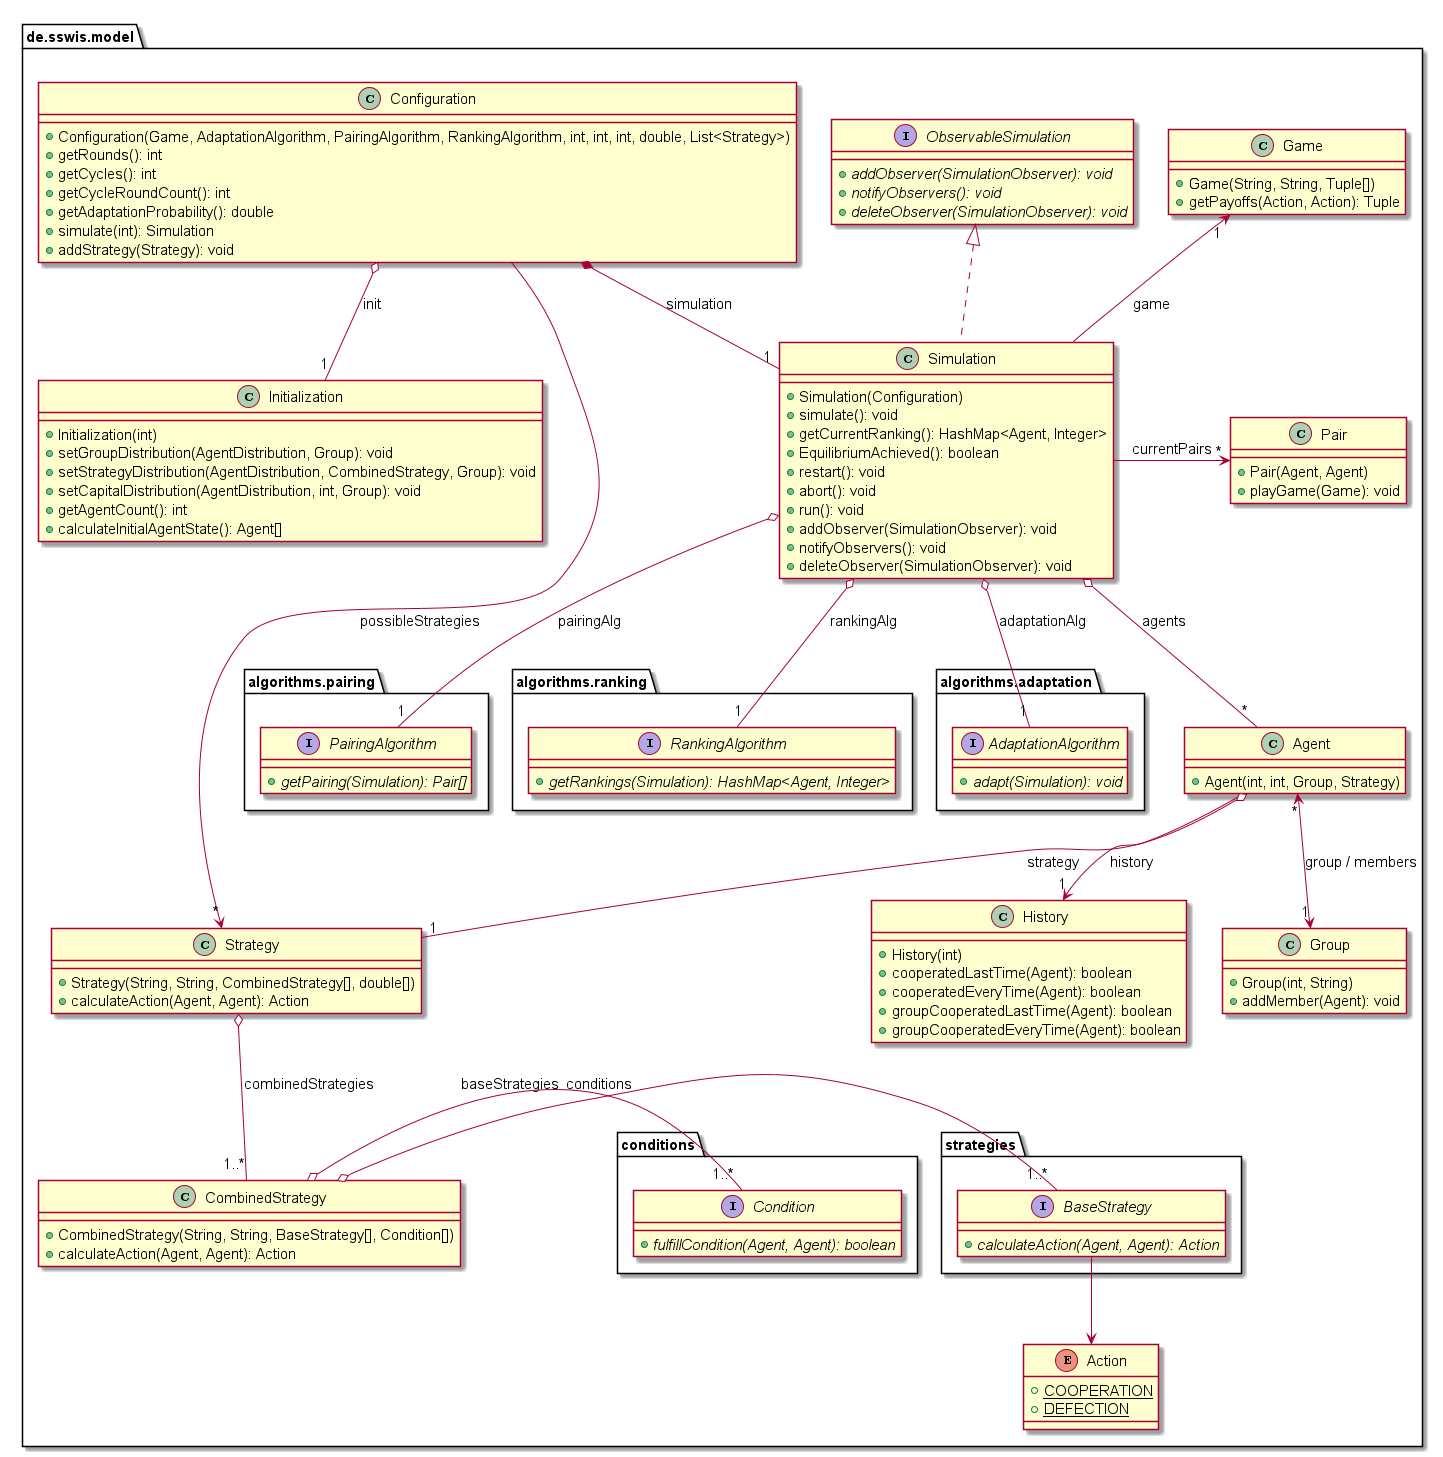
\includegraphics[scale=0.4]{model_classDiagramm}}

%TODO Beschreibung

\subsection{View}

\noindent
\makebox[\textwidth]{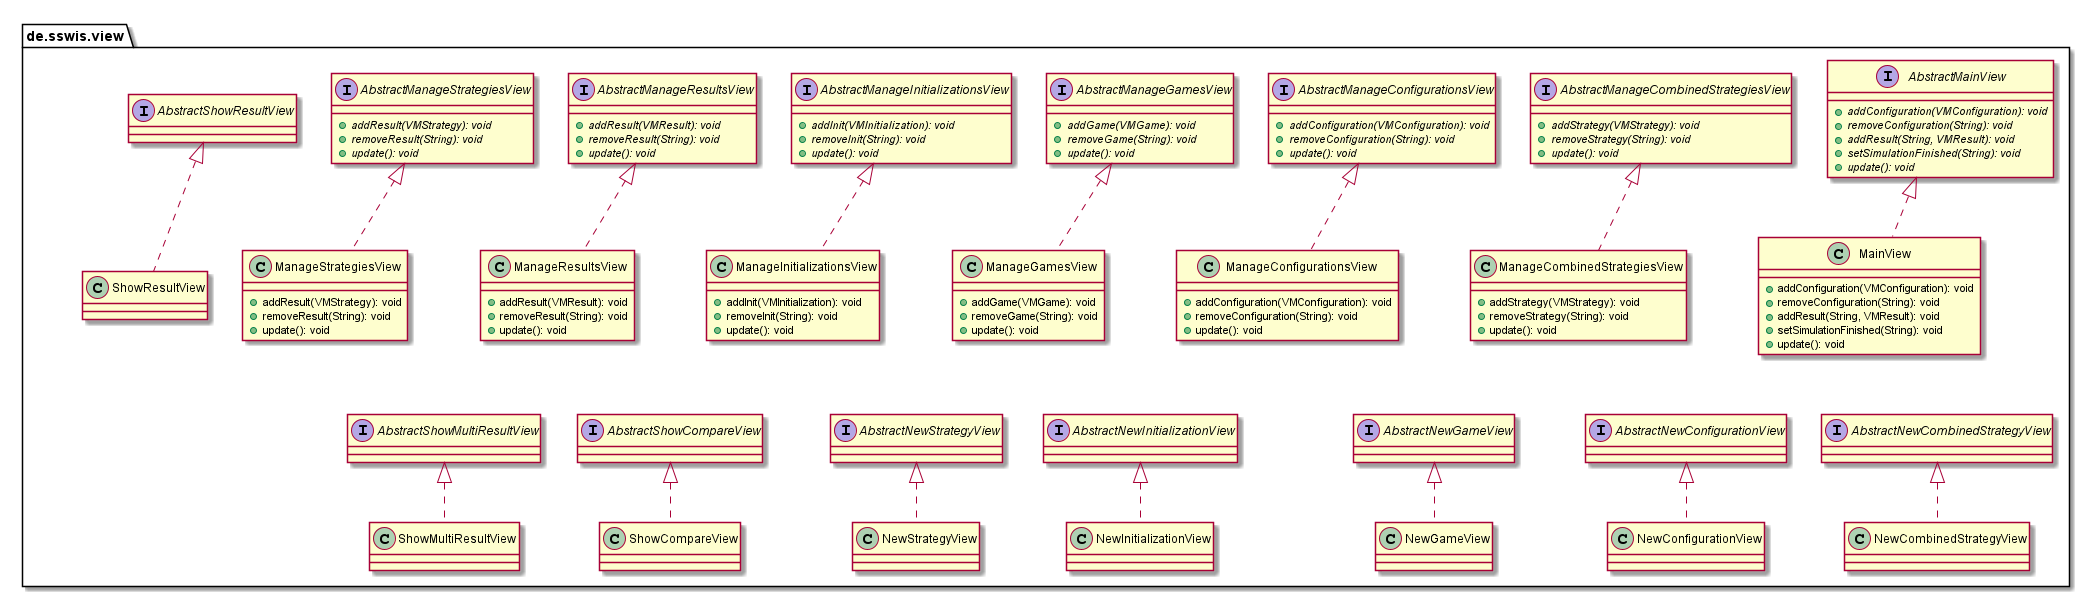
\includegraphics[scale=0.4]{view_classDiagramm}}

Für die Implementierung der Benutzeroberfläche wird die Java Swing Bibliothek und IntelliJ GUI Forms verwendet. In der View stehen alle Fenster, mit denen der Benutzer interagiert, als eigene Klasse zur Verfügung. Zur Übersicht sind nur drei dieser Klassen in dem Bild dargestellt, um das Zusammenspiel von View und View Model Objekten anschaulich zu machen. 

Die Fenster enthalten Buttons und Menuitems, mit denen der Nutzer interagieren kann. Für diese werden die Handler aus dem Controller als ActionListener gesetzt. 

Das Interface AbstractView enthält die grundlegendsten Methoden für ein GUI Fenster, um dieses anzeigen und schließen zu lassen. Jedes Fenster der Benutzeroberfläche implementiert ein eigenes Interface, das von AbtractView erbt und öffentliche Methoden, wie zum Beispiel zum Setzen der Actionlistener, enthält. 

MainView ist das Hauptfenster des Programms. Es zeigt alle Konfigurationen an und über Buttons kann eine ausgewählte Konfiguration gestartet und die Ergebnisse angezeigt und gespeichert werden. Dafür besitzt das Fenster eine Liste aller gespeicherten VMConfiguration Objekte.
Über das Menü kann der Nutzer sich alle Fenster zum Verwalten und Erstellen von Konfigurationen, Initialisierungen, Stufenspielen und gemischten und kombinierten Strategien öffnen lassen.

ManageGamesView ist ein Fenster zum Verwalten von Stufenspielen. Über Buttons können Stufenspiele bearbeitet, gelöscht und erstellt werden. Damit Informationen zu allen Stufenspielen angezeigt werden können, besitzt das Fenster eine Liste aller gespeicherten VMGame Objekte.

NewGameView ist ein Fenster zum Erstellen oder Bearbeiten eines Stufenspiels. Es besitzt ein VMGame Objekt, in das die Nutzereingaben übertragen werden. Das VMGame Objekt prüft dabei die Eingaben auf Korrektheit.

